\documentclass{book}
\usepackage[
HomeHTMLFilename=index,% Filename of the homepage.
HTMLFilename={node-},% Filename prefix of other pages.
mathjax,%Use MathJax to display math.
latexmk
]{lwarp}
\usepackage{lipsum}

\usepackage[spanish]{babel}
\usepackage{csquotes}
\usepackage{graphicx}

\usepackage{backref}
\usepackage{hyperref}

\boolfalse{FileSectionNames}% If false, numbers the files.
\renewcommand{\linkhomename}{Inicio}
\renewcommand{\linkpreviousname}{Anterior}
\renewcommand{\linknextname}{Siguiente}
\renewcommand{\sidetocname}{Sumario}
\setcounter{tocdepth}{2}% Include subsections in the \TOC.
\setcounter{secnumdepth}{2}% Number down to subsections.
\setcounter{FileDepth}{1}% Split \HTML\ files at sections
\setcounter{FootnoteDepth}{1}
\booltrue{CombineHigherDepths}% Combine parts/chapters/sections
\setcounter{SideTOCDepth}{1}% Include subsections in the side\TOC
\HTMLTitle{Título del libro}% Overrides \title for the web page.
\HTMLAuthor{Alberto Moyano}% Sets the HTML meta author tag.
\HTMLLanguage{es-ES}% Sets the HTML meta language.
\HTMLDescription{Lectura de notas}% Sets the HTML meta description.
\HTMLFirstPageTop{Título del libro}
\HTMLPageTop{
\includegraphics[width=2cm]{logo-imago-cmyk.png}}
\HTMLPageBottom{Información de contacto y legales (\url{https://www.edicionesimagomundi.com/})}
\CSSFilename{lwarp_custom.css}

\begin{document}
\frontmatter

\tableofcontents

\chapter{Portada}

Resolver un diseño de página tal que aparezca la tapa y los datos de catalogación.

\chapter{Frontmatter}

\lipsum[1]

\emph{Nulla malesuada porttitor diam}. Donec felis erat, congue non, volutpat at, tincidunt tristique, libero. Vivamus viverra fermentum felis. Donec nonummy pellentesque ante. Phasellus adipiscing semper elit. Proin fermentum massa ac quam. Sed diam turpis, molestie vitae, placerat a, molestie nec, leo. Maecenas lacinia. Nam ipsum ligula, eleifend at, accumsan nec, suscipit a, ipsum. Morbi blandit ligula feugiat magna. Nunc eleifend consequat lorem. Sed lacinia nulla vitae enim. Pellentesque tincidunt purus vel magna. Integer non enim. Praesent euismod nunc eu purus. Donec bibendum quam in tellus. Nullam cursus pulvinar lectus. Donec et mi. Nam vulputate metus eu enim. Vestibulum pellentesque felis eu massa.\footnote{\emph{Nulla malesuada porttitor diam}. Donec felis erat, congue non, volutpat at, tincidunt tristique, libero. Vivamus viverra fermentum felis. Donec nonummy pellentesque ante. Phasellus adipiscing semper elit.}

\lipsum[1]

\mainmatter

\chapter{Mainmatter}
\label{mychapter}

\lipsum[1]

\section{Title}

Lorem ipsum dolor sit amet, consectetuer adipiscing elit. Ut purus elit, vestibulum ut, placerat ac, adipiscing vitae, felis. Curabitur dictum gravida mauris. Nam arcu libero, nonummy eget, consectetuer id, vulputate a, magna. Donec vehicula augue eu neque. Pellentesque habitant morbi tristique senectus et netus et malesuada fames ac turpis egestas. Mauris ut leo. Cras viverra metus rhoncus sem. Nulla et lectus vestibulum urna fringilla ultrices. Phasellus eu tellus sit amet tortor gravida placerat. Integer sapien est, iaculis in, pretium quis, viverra ac, nunc. Praesent eget sem vel leo ultrices bibendum. Aenean faucibus. Morbi dolor nulla, malesuada eu, pulvinar at, mollis ac, nulla. Curabitur auctor semper nulla. Donec varius orci eget risus. Duis nibh mi, congue eu, accumsan eleifend, sagittis quis, diam. Duis eget orci sit amet orci dignissim rutrum.\footnote{\lipsum[3]}

\lipsum[1]

\begin{figure}[!ht]
	\centering
	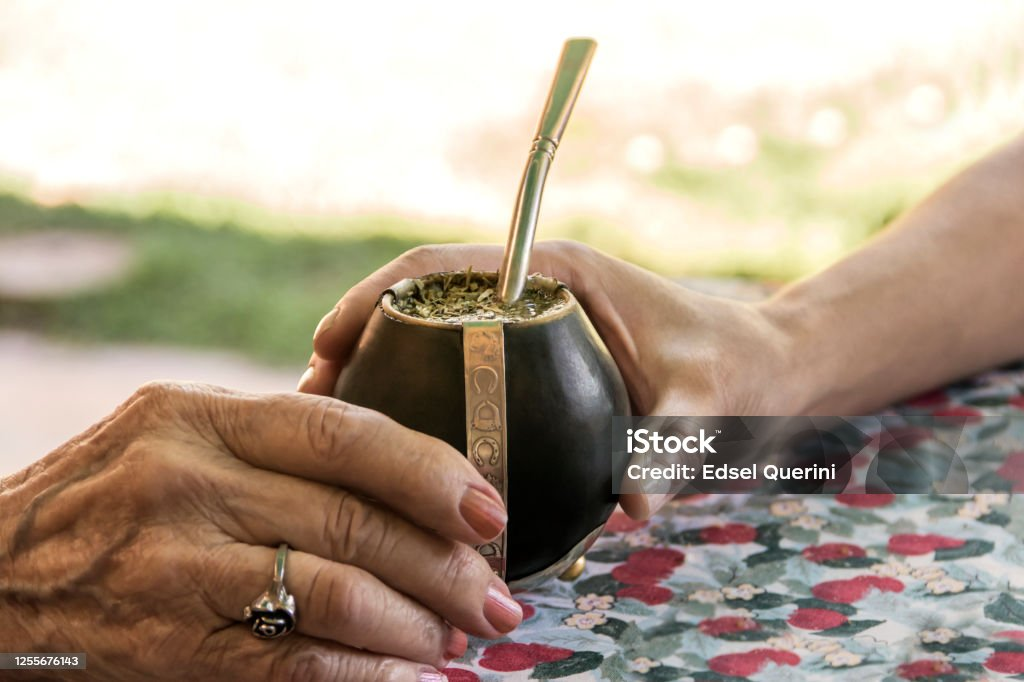
\includegraphics[width=\textwidth]{imagen1.jpg}
	\caption{Este es el epígrafe de la figura a color.}\label{figura1}
\end{figure}

\section{Title section}

\begin{enumerate}
	\item primero
	\item segundo
	\item tercero
\end{enumerate}

\lipsum[3]

\begin{quote}
	\enquote{Lorem ipsum dolor sit amet, consectetuer adipiscing elit. Ut purus elit, vestibulum ut, placerat ac, adipiscing vitae, felis. Curabitur dictum gravida mauris. Nam arcu libero, nonummy eget, consectetuer id, vulputate a, magna. Donec vehicula augue eu neque. Pellentesque habitant morbi tristique senectus et netus et malesuada fames ac turpis egestas}.
\end{quote}

\lipsum[5]

\section{Title section}

\lipsum[1]

\chapter{next meeting}
\label{mychapter2}

\section{Title section}

\lipsum[1]

\lipsum[1]

Como vemos en la figura \ref{figura1}, lorem ipsum dolor sit amet.\footnote{\lipsum[1]}

\lipsum[1]

\lipsum[1]

Como vemos en la figura \ref{figura1}, lorem ipsum dolor sit amet.\footnote{\lipsum[1]}

\lipsum[1]

\lipsum[2]

\section{Title section}

\lipsum[3]

\section{Title section}

\lipsum[1]

\subsection{Title section}

\lipsum[1]

\chapter{and next meeting}
As discussed in \ref{mychapter2}, lorem ipsum dolor sit amet.

\lipsum[2]

\section{Title section}

\lipsum[3]

\subsection{Title section}

\lipsum[1]

\backmatter

\chapter{Legales}

\lipsum[4]

\chapter{Colofón}

\lipsum[4]


\end{document}
